\item[(b)]
\section{Pole-Zero Map}

\subsection*{Problem Statement}
Draw a sketch of the pole-zero map.

\subsection*{Theoretical Background}
A pole-zero map is a graphical representation of the locations of the poles and zeros of a transfer function in the complex plane. Poles are typically represented by 'x' marks and zeros by 'o' marks.

\subsection*{Pole-Zero Map}
The given zeros are:
\begin{itemize}
    \item \( N_{1} = -1 \)
    \item \( N_{2} = j \)
    \item \( N_{3} = -j \)
\end{itemize}

The given poles are:
\begin{itemize}
    \item \( P_{1} = 0 \)
    \item \( P_{2} = 0.75 + j0.25 \)
    \item \( P_{3} = 0.75 - j0.25 \)
\end{itemize}

\begin{figure}[h]
    \centering
    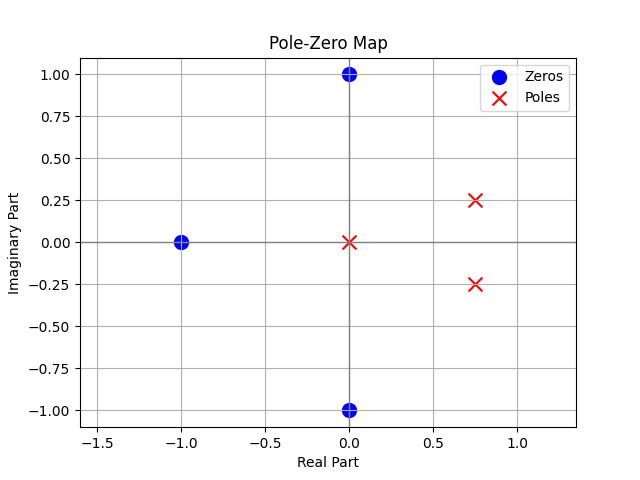
\includegraphics[width=0.8\textwidth]{fig/ex3_b_pole_zero_map.png}
    \caption{Pole-Zero Map}
    \label{fig:ex3_b_pole_zero_map}
\end{figure}

\subsection*{Conclusion}
The pole-zero map shows the locations of the poles and zeros in the complex plane. The zeros are marked with 'o' and the poles with 'x'.
